\chapter{Exercise Recommendation System Based on Knowledge State }

% **************************** Define Graphics Path **************************
\ifpdf
  \graphicspath{{Chapter4/Figs/Raster/}{Chapter4/Figs/PDF/}{Chapter4/Figs/}}
\else
  \graphicspath{{Chapter4/Figs/Vector/}{Chapter4/Figs/}}
\fi

\section{Motivation}



%自适应学习是指学习者根据学习内容的不同,选择不同的学习方式,在学习中 不断发现,最终找到符合自己的“个性化”学习方式。自适应学习不是简单的将线下资源搬到线上,也不是简单的“互联网+教育”的结合,而是注重以学生个体为 中心,对具有不同认知水平、不同认知风格的人提供不同的个性化学习方案。

%自适应学习概念一直是教育界研究的热点,也是很多教育学家研究的理论之 一。自从 Brusilovsky 提出自适应学习系统的通用模型开始,自适应学习概念才第一 次应用到工程实践当中,但是一直缺乏标准的参考模型和架构体系,直到第一个被 开发出来的自适应超媒体应用模型,到后来有 LAOS、XML 自适应媒体模型和WebXML 参考模型,自此,完成了自适应学习从教育界理论研究向计算机领域的 应用开发转变,众多自适应学习模型都将关注点聚焦在领域模型、学生模型和自适 应引擎的构建上。

%领域模型主要是构建学生的学习资源,此处的学习资源不是单纯的学生教材、 辅导资料,而是将该领域知识中的各个实体进行有结构化的组织,以本体或语义网 的形式来构建实体之间的关联,形成完备的知识库,其中实体主要包括细粒度的知 识点概念及其属性、例题、习题、资料甚至图形图像和音频等。

%学生模型主要是用来构建具有学生个体特征的模型,可以描述为学生个体对 领域模型中每个试题的掌握情况,学生模型会随着领域模型中实体关系的变化而 转变,学生个体特征还包括了学生个体的兴趣偏好、测试成绩、认知能力和知识水 平等。除此之外,根据我国教育技术规范关于学习者规范模型 CELTS-11中也对学 生模型进行了描述,增加了学生的年龄、背景、地区等额外信息。

%自适应引擎又被称为教学选择策略,通过对领域模型到学生模型的自适应解 释规则,实现能够根据学生的个性特征,由系统通过相关规则或是算法选择出满足 学生要求的领域模型供学生学习。目前较为流行的是运用大数据技术,通过统计学 生学习的路径或习惯,采用协同过滤推荐、内容推荐、混合推荐等流行的推荐算法, 推荐学生个性化的学习方案。

%本文在深入理解自适应参考模型后,进一步优化了模型中领域模型、学生模型、 教学策略,并将优化后的模型运用到构建智能题库系统上。将特征题库按照遗忘度、 抽象度、间接度、综合度、计算复杂度等维度进行信息结构化分类,学生个体通过 训练实时生成反映学生知识掌握能力的个体特征库。运用智能选题算法以个体特 征库为基础,动态从题库中智能选取切合个体的训练集。

High school mathematics intelligent question bank is built by learning from the model of adaptive learning. Adaptive learning is the theoretical abstraction of adaptive learning system model. Many adaptive learning system models focus on the construction of domain model, student model and adaptive engine. This paper proposes an intelligent recommendation algorithm based on individual characteristics, which integrates domain model, student model and adaptive engine The self-adaptive engine abstracts the high school mathematics question bank into the characteristic question bank according to the domain model, and abstracts the student model into the individual characteristic bank. The self-adaptive engine is based on the individual characteristic bank through the intelligent algorithm, dynamically selects the training questions suitable for the individual from the characteristic question bank, and realizes the personalized recommendation of the question bank.

Traditional paper teaching materials are usually printed in large quantities. Due to the limitation of paper space and in order to adapt to the majority of students, one or two representative test questions have to be selected according to each chapter. In order to meet the comprehensiveness of knowledge points and the public adaptability, such teaching aids lead to the small scale of test questions, the incomplete coverage of questions and the failure to meet the requirements of students' targeted training. E-learning has brought a reform in the field of teaching with its flexible learning style, avoiding large class teaching, and students can choose their own learning resources through autonomous navigation. Online question bank with eleaning As the times require, the early online question bank simply moves the offline resources to the Internet. Although students can choose their own topics and find the test questions they want for intensive training, it is lack of interactivity. Students do not get timely and effective feedback after finishing the questions, and can not accurately locate the strengths and weaknesses of students, which is very limited in improving students' performance. In view of these shortcomings, it is the current research direction of intelligent question bank to build a student-centered system, in which students can feed back their mastery of knowledge points in real time by doing questions, and build a complete user portrait of students. The question bank can intelligently diagnose, screen and push targeted questions according to the submission of students' questions.

Adaptive learning means that learners choose different learning styles depending on the content they are learning, and that they continue to discover their own "personalized" learning style as they learn. Adaptive learning is not a simple transfer of offline resources to online, nor is it a simple combination of "Internet + education". Rather, it focuses on the individual student and provides different personalized learning programs for people with different cognitive levels and styles.

The concept of adaptive learning has been a hot topic of research in the education field and has been one of the theories studied by many educators. Since Brusilovsky proposed a general model of adaptive learning system, the concept of adaptive learning was first applied to engineering practice, but there has been a lack of standard reference models and architectural systems until the first adaptive hypermedia application model was developed, and later there were LAOS, XML adaptive media model and WebXML reference model.
Since then, adaptive learning has been transformed from theoretical research in education to application development in computing, and many adaptive learning models have focused on the construction of domain models, student models, and adaptive engines.

The domain model focuses on building student learning resources, which are not just student textbooks or tutorials, but also structured entities in the domain knowledge, and ontologies or semantic webs are used to build connections between entities to form a complete knowledge base, including fine-grained knowledge concepts and their attributes, examples, exercises, materials, and even graphical images and audio.

The student model is mainly used to build a model with individual student characteristics, which can be described as individual students' mastery of each test topic in the domain model, and the student model will change with the changes of entity relationships in the domain model. In addition, the student model is also described in CELTS-11 according to our educational technology specification on the learner specification model, which adds additional information such as the student's age, background, and region.

The adaptive engine, also known as the instructional selection strategy, uses adaptive interpretation rules from the domain model to the student model to enable the system to select the domain model that meets the student's requirements based on the student's personality characteristics, either through rules or algorithms. Currently, it is popular to use big data technology to recommend students' personalized learning solutions by using popular recommendation algorithms such as collaborative filtering recommendation, content recommendation, and hybrid recommendation through statistics of students' learning paths or habits.

In this paper, we further optimize the domain model, student model, and teaching strategy in the adaptive reference model, and apply the optimized model to build an intelligent question bank system. The feature database is structured according to the dimensions of forgetfulness, abstractness, indirectness, comprehensiveness, and computational complexity, and individual students are trained to generate a database of individual features reflecting their knowledge acquisition ability in real time. The intelligent question selection algorithm is used to dynamically select the appropriate training set from the question database based on the individual feature database.

\section{Proposed Model}
\subsection{Algorithm Overview}
% 本章提出一个结合图神经网络知识追踪和协同过滤的试题自适应推荐方法。该方法通过上一章设计的基于GAT知识追踪模型模型对学生的知识状态进行建模,并利用图神经网络的聚类方法来对试题进行基于知识点的聚类,从而可以获取一系列相关的习题。分为以下几个部分,第一部分为召回部分,即候选试题生成,它产生一系列相似的习题,这是通过图神经网络来对试题进行聚类来进行,它应用图聚类方法,将试题基于知识点来进行合理聚类。第二部分为排序部分,它结合知识追踪系统获取的学生的知识状态,并结合协同过滤算法,来生成一个Top N的习题推荐列表;第三部分为反馈部分,学生做的推荐的习题又回继续输入到知识追踪系统和推荐系统中。
%1. 练习候选生成。这部分的作用是生成一系列符合学生当前学习状态的练习,并快速筛选出一组初步的练习,后续部分将从这组练习中生成最合适的N个练习,并通过协同过滤算法进行排序。它参考youtube推荐系统设计了一个多层MLP网络。它将知识跟踪生成的学生学习状态嵌入向量与学生的问题记录嵌入、个性化信息等并联作为输入。经过一系列的ReLU网络,然后通过softmax归一化输出所有候选练习的概率分布。
%2. 第二部分该部分用与上一部分类似的神经网络架构,实现了对推荐试题的排序。它的输入是用户的知识结构,最近练习,以及相似用户的常见练习题。

This chapter proposes an adaptive recommendation method for test questions that combines graph neural network knowledge tracking and collaborative filtering. The method models students' knowledge states through the GAT-based knowledge tracking model model designed in the previous chapter, and uses the clustering method of graph neural networks to perform knowledge-based clustering of test questions so that a series of relevant exercises can be obtained. The first part is the recall part, i.e., candidate test generation, which generates a series of similar exercises, and this is done by clustering the test questions through graph neural networks, which apply graph clustering methods to cluster the test questions based on knowledge points in a reasonable way. The second part is the ranking part, which combines the knowledge state of students obtained from the knowledge tracking system with co-filtering.
\begin{enumerate}
  \item Exercise candidate generation: The role of this part is to generate a series of exercises that match the student's current learning state, and quickly filter out a preliminary set of exercises, and the subsequent part will generate the most suitable N exercises from this set and sort them by collaborative filtering algorithms. It designs a multi-layer MLP network with reference to the youtube recommendation system. It concatenates the student learning state embedding vector generated by knowledge tracking with the student's problem record embedding, personalized information, etc. as input. After a series of ReLU networks and then output a probability distribution over all candidate exercises by softmax normalization.
  \item Ranking: This part is to generate Top N recommendation exercise. It implements the ranking of the recommended test questions using a neural network architecture similar to that of the previous section. Its inputs are the user's knowledge structure, recent exercises, and common practice questions from similar users.
\end{enumerate}

The structure of the recommendation system is like Figure. \ref{fig0}

\begin{figure}[h]
  \centering
  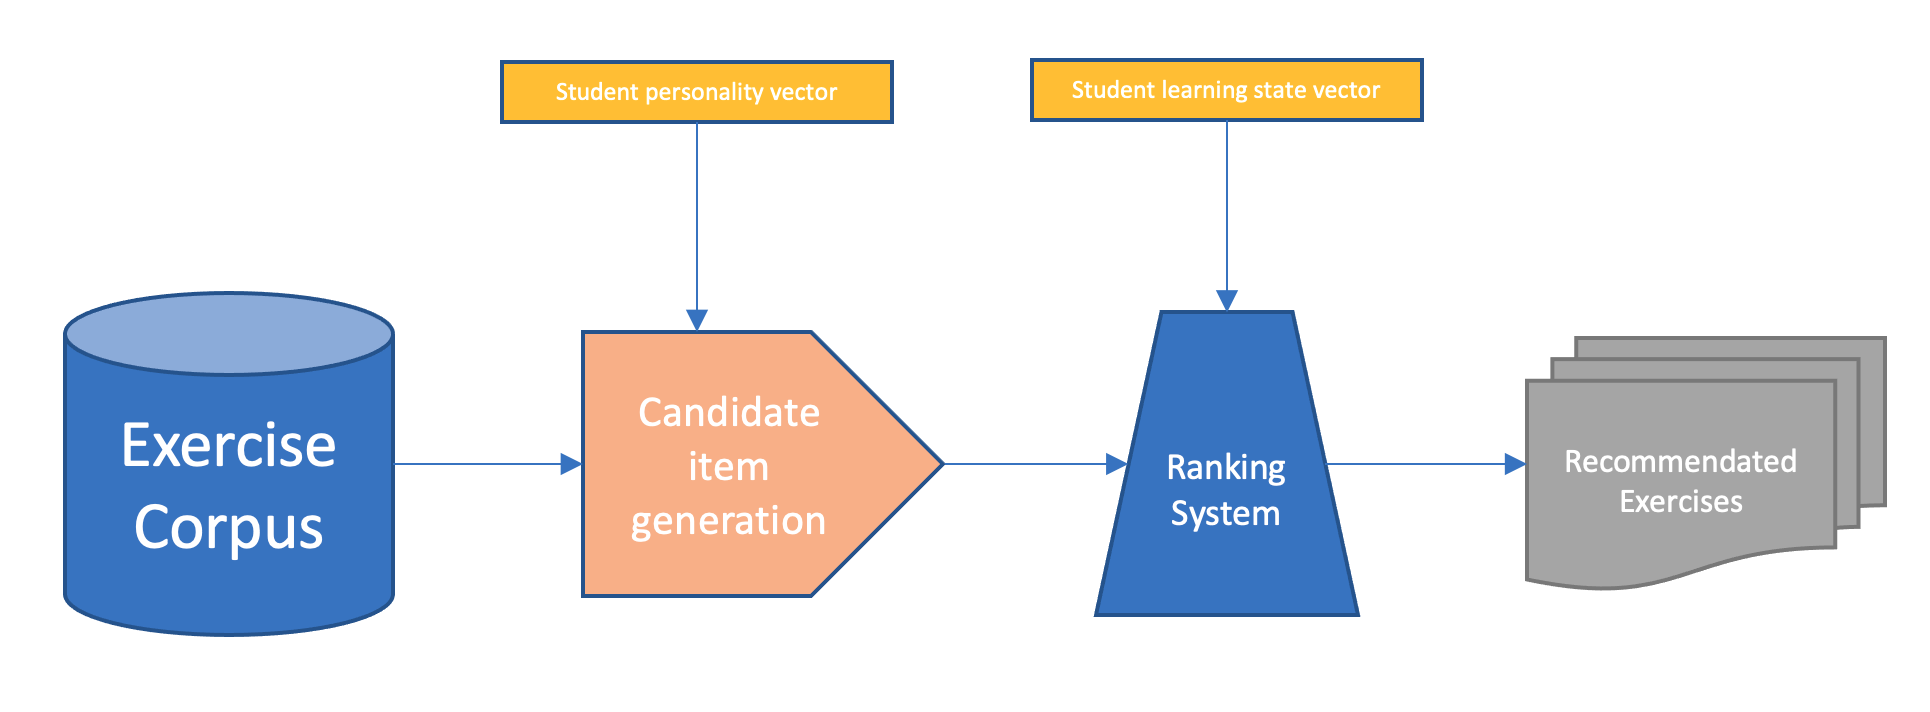
\includegraphics[width=1.0\textwidth]{ch4-fig1.png}
  \caption{The Architecture of Recommendation System}
  \label{fig0}
\end{figure}

\subsection{Recall Stage}
In the recall phase, due to the large amount of data, the algorithm of Collaborative Filtering (CF) can achieve half the result with twice the effort. It only needs to calculate the similarity of students' knowledge states $h^\prime$ with other students who have similar knowledge states $h$.

Collaborative Filtering, the most classic type of recommendation algorithm, includes both online collaborative and offline filtering. The so-called online collaborative is to find items that users may like through online data, while offline filtering is to filter out data that are not worth recommending, such as data with low recommendation value ratings, or data that users have already purchased despite high recommendation values. The model of collaborative filtering is generally m recommended items, m users' data, only some users and some data are rated between the data, other parts of the rating is blank, at this time we want to use the existing part of the sparse data to predict the rating relationship between those blank items and data to find the highest rated items recommended to users.

Generally speaking, there are three types of collaborative filtering recommendations. The first one is user-based collaborative filtering, the second one is item-based collaborative filtering, and the third one is model-based collaborative filtering.


\subsubsection{Student Similarity Calculation}
The purpose of collaborative filtering is to recommend recommended items of users similar to the target user to the user. The user-based collaborative filtering algorithm is discovered through historical behavior data of users, and measures and scores these preferences. Set the similarity of users through a given algorithm, and make recommendations among users who have the same preferences.

User-based collaborative filtering mainly considers the similarity between users and users. As long as we find out the items that similar users like and predict the target users' ratings of the corresponding items, we can find the items with the highest ratings and recommend them to users. The item-based collaborative filtering is similar to the user-based collaborative filtering, except that we turn to find the similarity between items and users, and only if we find the ratings of certain items by target users, then we can predict similar items with high similarity and recommend the highest rated similar items to users. For example, if you buy a machine learning related book online, the website will immediately recommend a bunch of machine learning, big data related books to you, and the idea of collaborative filtering based on items is obviously used here.

Similar statistics are used to get neighboring users with similar hobbies or interests, so we can use the obtained user's knowledge state embedding $h_t$ from the previous knowledge tracking module, which can be used as the basis for calculating the similarity. The first step is to find other users who are similar to the new user based on their historical behavior information; at the same time, to predict the items that the current new user may like based on the evaluation information of these similar users on other items. Given the user rating data matrix R, the user-based collaborative filtering algorithm needs to define the similarity function $s : U \times U \to R$ to calculate the similarity between users, and then calculate the recommendation results based on the rating data and the similarity matrix. We can use the cosine similarity to calculate this value.

\begin{align}
  s(u, v)=\frac{h_{u} \cdot h_{v}}{\left\|h_{u}\right\|_{2}\left\|h_{v}\right\|_{2}}
\end{align}
where $h_u$ and $h_v$ represent the knowledge mastery state of user $u$ and $v$.
We can obtain the exercise recommendation history \mathcal{H} of user B, which is closest to user A to be recommended, and then use the exercises in \mathcal{H} as a rough set as the next sorted list of exercises.

\subsubsection{Exercise Filtering System}
Through the previous section, we calculated the similarity of students, which comprehensively considers students’ current knowledge proficiency, students’ personalized information and so on. Next, we need to use the collaborative filtering algorithm to generate a rough recommended set of exercises $S_{raw}$.

When the recommendation system is running, the system will record the students’ question records. After calculating the similarity of the students, they can be sorted according to the similarity. Given a threshold, list the students whose similarity is greater than the threshold, and divide the students according to the list. The exercises corresponding to the problem record are added to $S_{raw}$.

The algorithm is as \ref{alg:EF}:
\begin{algorithm}[h]
  \caption{Exercise Filtering Algorithm}
  \label{alg:EF}
  \begin{algorithmic}
    \REQUIRE ~~\\
    The target student $s_i$; \\
    The student represent matrix, $S=\{s_0,s_1,...,s_N\}$;\\
    The log of recommendation $L=\{L_0,L_1,...,L_N\}$ \\
    The log-exercise relation: $L_i=\{E_0,...,E_{|L_i|}\}$\\
    The filtering thread $T$;
    \ENSURE ~~\\ %算法的输出:Output
    The filted exercise set $S={E_{s_0},...,E_{s_{N^'}}}$
    \STATE Calculate the similarity between $s_i$ and other students $Sim$
    \STATE Sort $Sim$ and get the top $T$ results $R=\{s_{r_0},...,s_{r_T}\}$;
    \STATE Aggregate the exercises log of students in $R$, get exercise set $S$
    \RETURN $S$; %算法的返回值
  \end{algorithmic}
\end{algorithm}




\subsection{Ranking Stage}
%本节我们设计了一个基于MLP的试题排序模型,该模型输入学生的知识状态向量$h_t$,以及通过序列嵌入学习的知识状态改变向量$d_h$,以及习题的知识点标注向量。

In the previous step we obtained a list of recommended exercises for similar students by collaborative filtering in the recall phase, and in this phase, a ranking of the exercises is needed to further reduce the amount of recommendations and give the ranking sequence of exercise. In this section, we design an MLP-based test ordering model. The model inputs the student's knowledge state vector $h_t$, the knowledge state change vector $d_h$ learned through sequence embedding, and the knowledge point labeling vector of the exercises. The architecture is like figure \ref{fig:ch4-fig3}.


\begin{figure}[h]
  \centering
  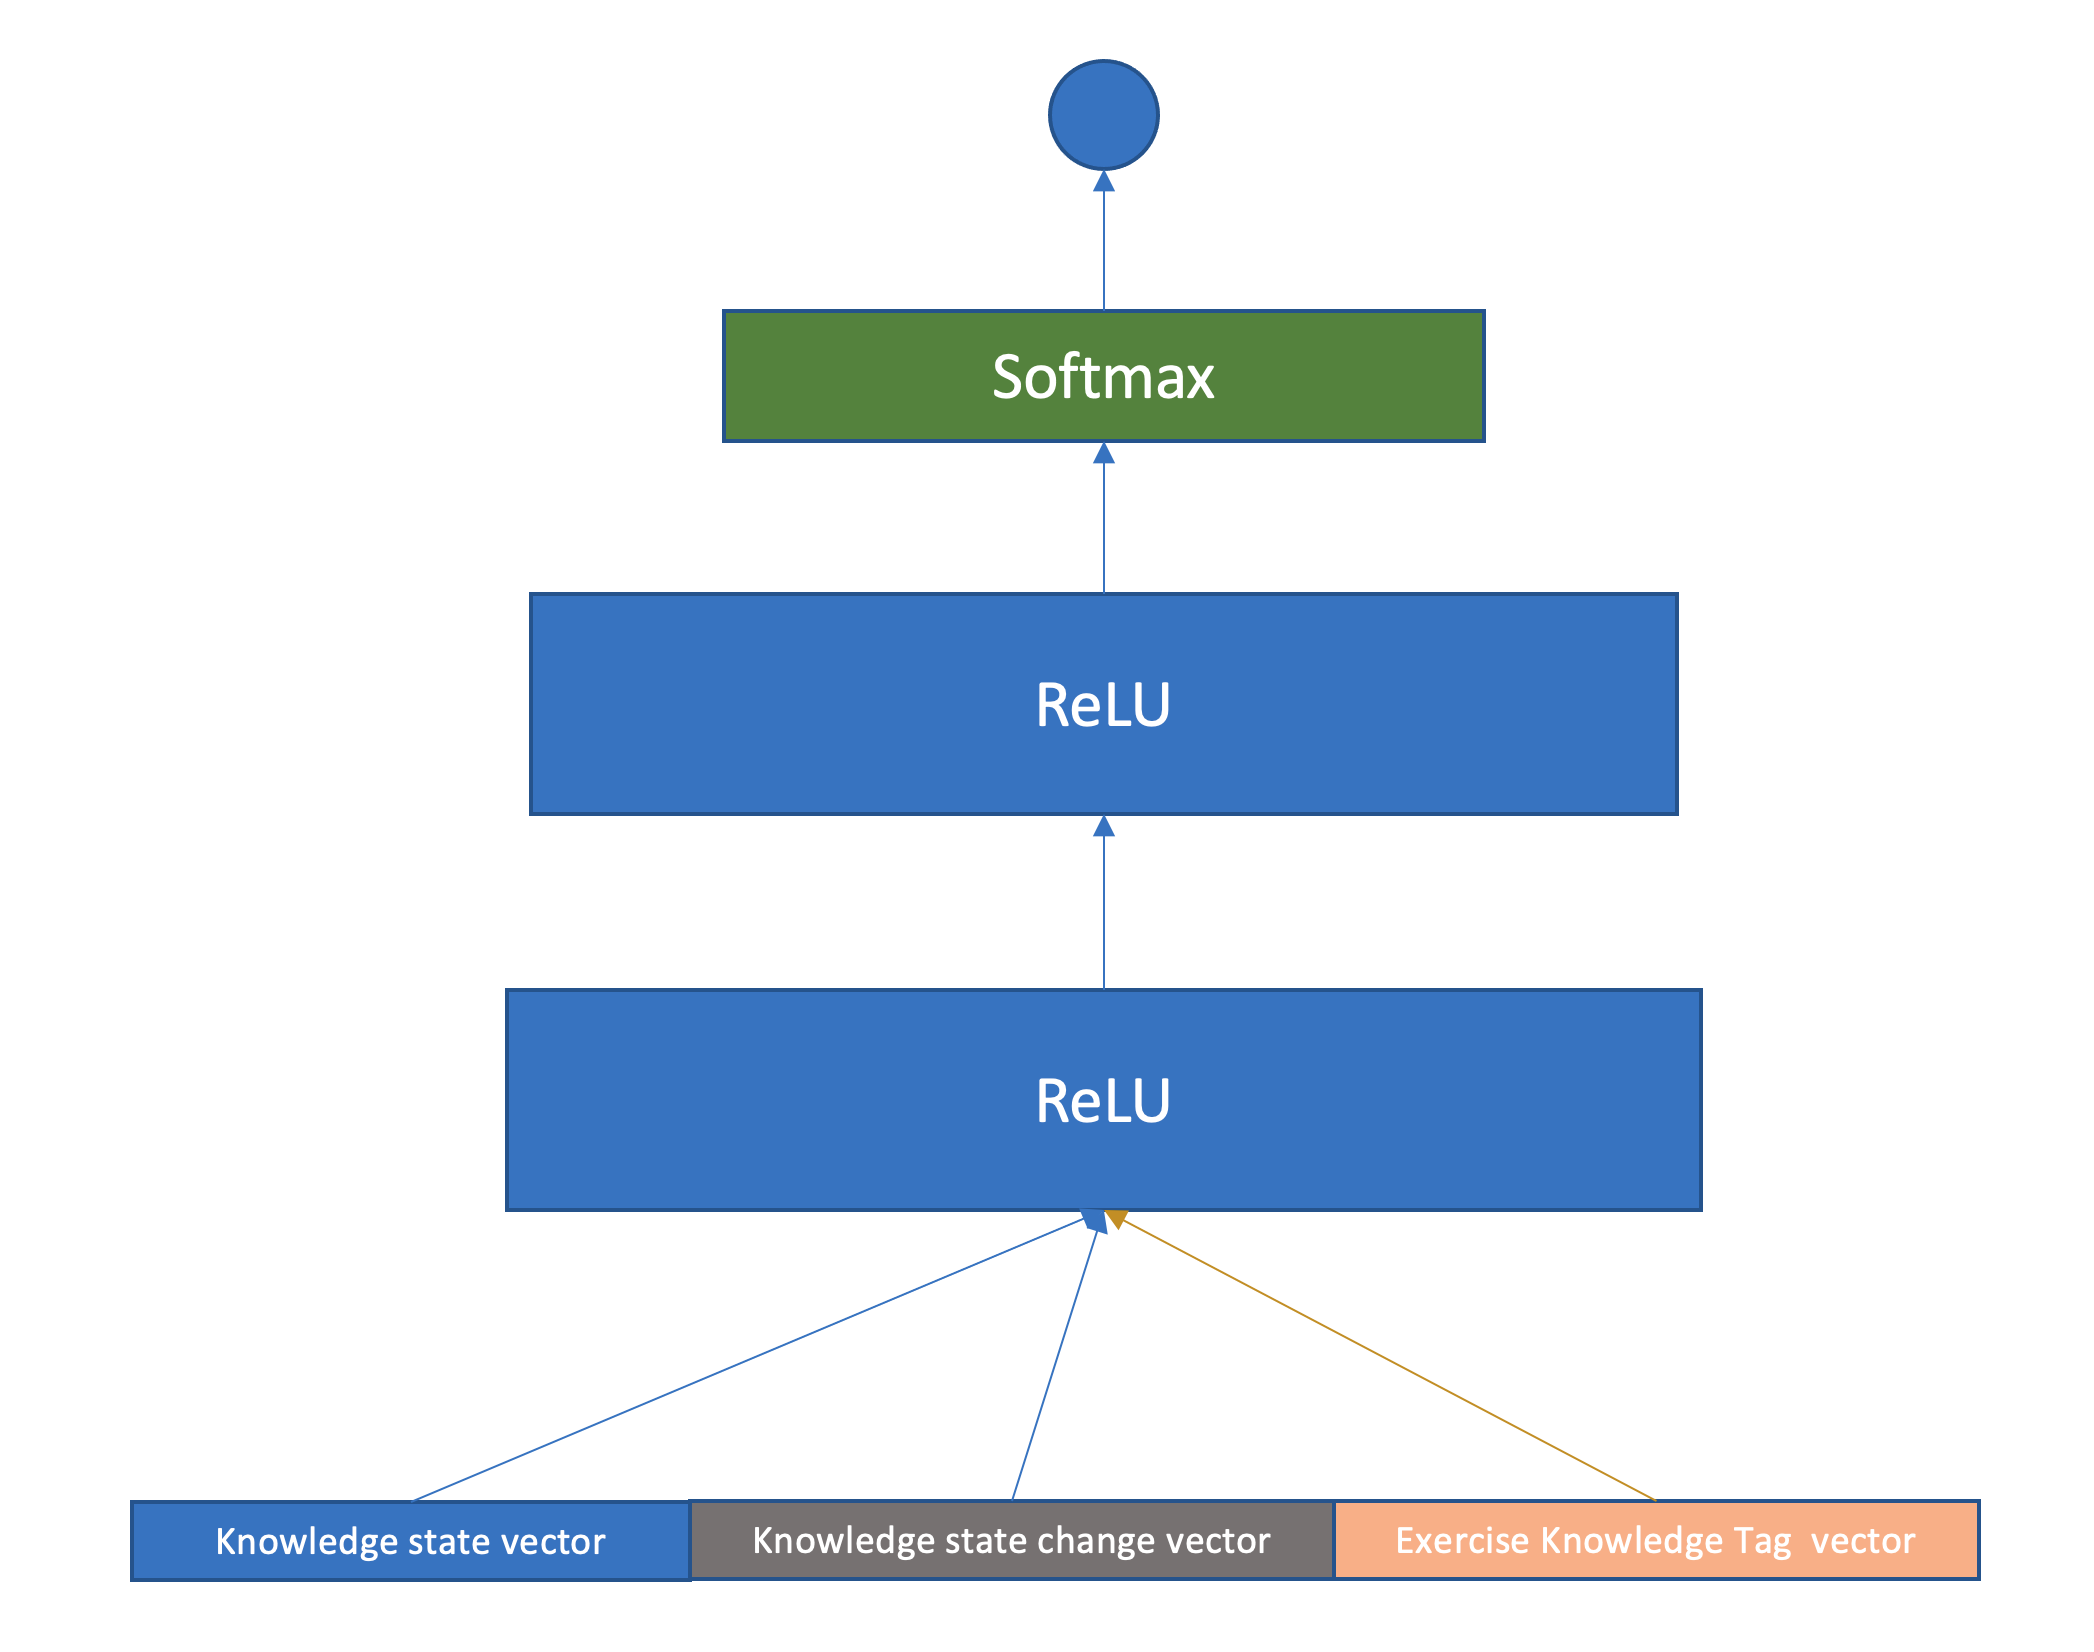
\includegraphics[width=1.0\textwidth]{ch4-fig3.png}
  \caption{The Architecture of Recommendation System}
  \label{fig:ch4-fig3}
\end{figure}

The model is a three-layer multi-layer perceptron, with two fully connected layers in the middle, and the output layer uses softmax to output the probabilities of exercise recommendation. The input layer inputs the student's knowledge state vector, knowledge state change vector and exercise knowledge point label vector. The model is a three-layer multi-layer perceptron, with two fully connected layers in the middle, and the output layer uses softmax to output the probabilities of exercise recommendation. The input layer inputs the student's knowledge state vector, knowledge state change vector and exercise knowledge point label vector. The loss function is:
\begin{align}
  \mathcal{L}=\sum_{i=1}^{T} y_i \log \left(\text{sigmoid}\left(\hat{y}_i\right)\right)+\left(1-y_i \right) \log (1-\text{sigmoid}(\hat{y}_i))
\end{align}
where $\hat{y}_i$ is the output value, $y_i$ is actual recommended weights for the exercises.

After training the model, sort the output values, and the sorted list is the recommended problem set.
%在训练好模型之后,将输出值进行排序,排序的列表即为推荐的习题集。
% \mynote{TODO:设计一个图神经网络用于知识点权重embedding or 简单的PMF等认知诊断算法} 
% \section{Experiment}

% \subsection{Database}
% \subsection{Baseline}
% \subsection{Result}

\section{Summary}
%本节提出了一个基于召回-排序的双阶段推荐系统框架,在召回阶段,采用了协同过滤的方式,排序阶段,则采用了多层感知机,来对学生知识状态-习题知识点进行建模,同时考虑到学生的学习速度即知识状态改变,输出习题与当前知识状态匹配度。
This section proposes a two-stage recommendation system framework based on recall-ranking. In the recall stage, collaborative filtering is used, and in the ranking stage, multi-layer perceptrons are used to model students' knowledge state-exercise knowledge points. At the same time, taking into account the student’s learning speed, that is, the change of knowledge state, the output exercises match the current knowledge state.